\chapter{Input variables with the best reconstruction improvement}
The following tables list all input variables, for which a top quark reconstruction improvement of more than \SI{4}{\%} was achieved by using the DNN classifier compared to the best-mass method introduced in Section \ref{sec:ch-5-best-mass}.

\begin{table}[h]
    \centering
    \label{tab:app_vars_1}
    \caption{}
    \begin{tabular}{ |c|@{}c@{}| }
        \hline
        \textbf{Improvement} & \textbf{Variables}\\
        \hline
        \SI{7.83}{\%} & 
        \begin{tabular}{ll}
            \hline
            Variable & Description\\
            \hline
            $p_T(j_1)$ & Transverse momentum of first jet\\
            $\eta(j_1)$ & Pseudorapidity of first jet\\
            $\phi(j_1)$ & $\phi$ of first jet\\
            $m_0(j_1)$ & Invariant mass of first jet\\

            $p_T(j_2)$ & Transverse momentum of second jet\\
            $\eta(j_2)$ & Pseudorapidity of second jet\\
            $\phi(j_2)$ & $\phi$ of second jet\\
            $m_0(j_2)$ & Invariant mass of second jet\\

            $\Delta R(j_1, w)$ & Distance between the first jet and the \PWplus boson\\
            $\Delta R(j_1, lep)$ & Distance between the first jet and the lepton\\
            $\Delta R(j_2, w)$ & Distance between the second jet and the \PWplus boson\\
            $\Delta R(j_2, lep)$ & Distance between the second jet and the lepton\\
            \hline
        \end{tabular}\\
        \hline
    \end{tabular}
\end{table}

\begin{table}[h]
    \centering
    \label{tab:app_vars_1}
    \caption{}
    \begin{tabular}{ |c|@{}c@{}| }
        \hline
        \textbf{Improvement} & \textbf{Variables}\\
        \hline
        \SI{5.02}{\%} & 
        \begin{tabular}{ll}
            \hline
            Variable & Description\\
            \hline
            $p_T(j_1)$ & Transverse momentum of first jet\\
            $\eta(j_1)$ & Pseudorapidity of first jet\\
            $\phi(j_1)$ & $\phi$ of first jet\\
            $m_0(j_1)$ & Invariant mass of first jet\\

            $p_T(j_2)$ & Transverse momentum of second jet\\
            $\eta(j_2)$ & Pseudorapidity of second jet\\
            $\phi(j_2)$ & $\phi$ of second jet\\
            $m_0(j_2)$ & Invariant mass of second jet\\

            $\Delta R(j_1, w)$ & Distance between the first jet and the \PWplus boson\\
            $\Delta R(j_2, w)$ & Distance between the second jet and the \PWplus boson\\

            $p_T(w)$ & Transverse momentum of the \PWplus boson\\
            $\eta(w)$ & Pseudorapidity of the \PWplus boson\\
            $\phi(w)$ & $\phi$ of the \PWplus boson\\
            $m_0(w)$ & Invariant mass of the \PWplus boson\\
            \hline
        \end{tabular}\\
        \hline
    \end{tabular}
\end{table}

\begin{table}[h]
    \centering
    \label{tab:app_vars_1}
    \caption{}
    \begin{tabular}{ |c|@{}c@{}| }
        \hline
        \textbf{Improvement} & \textbf{Variables}\\
        \hline
        \SI{4.77}{\%} & 
        \begin{tabular}{ll}
            \hline
            Variable & Description\\
            \hline
            $p_T(j_1)$ & Transverse momentum of first jet\\
            $\eta(j_1)$ & Pseudorapidity of first jet\\
            $\phi(j_1)$ & $\phi$ of first jet\\
            $m_0(j_1)$ & Invariant mass of first jet\\

            $p_T(j_2)$ & Transverse momentum of second jet\\
            $\eta(j_2)$ & Pseudorapidity of second jet\\
            $\phi(j_2)$ & $\phi$ of second jet\\
            $m_0(j_2)$ & Invariant mass of second jet\\

            $\Delta R(j_1, w)$ & Distance between the first jet and the \PWplus boson\\
            $\Delta R(j_1, lep)$ & Distance between the first jet and the lepton\\
            $\Delta R(j_2, w)$ & Distance between the second jet and the \PWplus boson\\
            $\Delta R(j_2, lep)$ & Distance between the second jet and the lepton\\

            $p_T(w)$ & Transverse momentum of the \PWplus boson\\
            $\eta(w)$ & Pseudorapidity of the \PWplus boson\\
            $\phi(w)$ & $\phi$ of the \PWplus boson\\
            $m_0(w)$ & Invariant mass of the \PWplus boson\\
            \hline
        \end{tabular}\\
        \hline
    \end{tabular}
\end{table}

\begin{table}[h]
    \centering
    \label{tab:app_vars_1}
    \caption{}
    \begin{tabular}{ |c|@{}c@{}| }
        \hline
        \textbf{Improvement} & \textbf{Variables}\\
        \hline
        \SI{4.52}{\%} & 
        \begin{tabular}{ll}
            \hline
            Variable & Description\\
            \hline
            $p_T(j_1)$ & Transverse momentum of first jet\\
            $\eta(j_1)$ & Pseudorapidity of first jet\\
            $\phi(j_1)$ & $\phi$ of first jet\\
            $m_0(j_1)$ & Invariant mass of first jet\\

            $p_T(j_2)$ & Transverse momentum of second jet\\
            $\eta(j_2)$ & Pseudorapidity of second jet\\
            $\phi(j_2)$ & $\phi$ of second jet\\
            $m_0(j_2)$ & Invariant mass of second jet\\

            $\Delta R(j_1, w)$ & Distance between the first jet and the \PWplus boson\\
            $\Delta R(j_2, w)$ & Distance between the second jet and the \PWplus boson\\

            $p_T(w)$ & Transverse momentum of the \PWplus boson\\
            $\eta(w)$ & Pseudorapidity of the \PWplus boson\\
            $\phi(w)$ & $\phi$ of the \PWplus boson\\
            $m_0(w)$ & Invariant mass of the \PWplus boson\\
            $m_T(w)$ & Transverse mass of the \PWplus boson\\
            \hline
        \end{tabular}\\
        \hline
    \end{tabular}
\end{table}

\begin{table}[h]
    \centering
    \label{tab:app_vars_1}
    \caption{}
    \begin{tabular}{ |c|@{}c@{}| }
        \hline
        \textbf{Improvement} & \textbf{Variables}\\
        \hline
        \SI{4.45}{\%} & 
        \begin{tabular}{ll}
            \hline
            Variable & Description\\
            \hline
            $p_T(j_1)$ & Transverse momentum of first jet\\
            $\eta(j_1)$ & Pseudorapidity of first jet\\
            $\phi(j_1)$ & $\phi$ of first jet\\
            $m_0(j_1)$ & Invariant mass of first jet\\

            $p_T(j_2)$ & Transverse momentum of second jet\\
            $\eta(j_2)$ & Pseudorapidity of second jet\\
            $\phi(j_2)$ & $\phi$ of second jet\\
            $m_0(j_2)$ & Invariant mass of second jet\\

            $\Delta R(j_1, w)$ & Distance between the first jet and the \PWplus boson\\
            $\Delta R(j_2, w)$ & Distance between the second jet and the \PWplus boson\\

            $p_T(w)$ & Transverse momentum of the \PWplus boson\\
            $\eta(w)$ & Pseudorapidity of the \PWplus boson\\
            $\phi(w)$ & $\phi$ of the \PWplus boson\\
            $m_0(w)$ & Invariant mass of the \PWplus boson\\
            $m_T(w)$ & Transverse mass of the \PWplus boson\\
            $met_T(w)$ & Transverse missing energy of the \PWplus boson\\
            \hline
        \end{tabular}\\
        \hline
    \end{tabular}
\end{table}

\begin{table}[h]
    \centering
    \label{tab:app_vars_1}
    \caption{}
    \begin{tabular}{ |c|@{}c@{}| }
        \hline
        \textbf{Improvement} & \textbf{Variables}\\
        \hline
        \SI{4.31}{\%} & 
        \begin{tabular}{ll}
            \hline
            Variable & Description\\
            \hline
            $p_T(j_1)$ & Transverse momentum of first jet\\
            $\eta(j_1)$ & Pseudorapidity of first jet\\
            $\phi(j_1)$ & $\phi$ of first jet\\
            $m_0(j_1)$ & Invariant mass of first jet\\

            $p_T(j_2)$ & Transverse momentum of second jet\\
            $\eta(j_2)$ & Pseudorapidity of second jet\\
            $\phi(j_2)$ & $\phi$ of second jet\\
            $m_0(j_2)$ & Invariant mass of second jet\\
            
            $p_T(w)$ & Transverse momentum of the \PWplus boson\\
            $\eta(w)$ & Pseudorapidity of the \PWplus boson\\
            $\phi(w)$ & $\phi$ of the \PWplus boson\\
            $m_0(w)$ & Invariant mass of the \PWplus boson\\

            $\Delta R(j_1, w)$ & Distance between first jet and the \PWplus boson\\
            $\Delta \phi(j_1, w)$ & $\phi$ difference between the first jet and the \PWplus boson\\
            $m_0(j_1, w)$ & Invariant mass of first jet and the \PWplus boson system\\
            
            $\Delta R(j_2, w)$ & Distance between the second jet and the \PWplus boson\\
            $\Delta \phi(j_2, w)$ & \phi difference between the second jet and the \PWplus boson\\
            $m_0(j_2, w)$ & Invariant mass of the second jet and the \PWplus boson system\\
            \hline
        \end{tabular}\\
        \hline
    \end{tabular}
\end{table}

\chapter{Plots of reconstruction improvement over average learning rate}
The following plots demonstrate how the average learning rate of the training of the classifier affects the reconstruction improvement in percent of the DNN over the best-mass method. The classifier topology and its input variables differ slightly in every training instance below. In one instance batch normalization was used. The logarithmic learning rate that yields the best improvement appears to be in the $10^{-6}$ order of magnitude.

\begin{figure}[h]
    \centering
    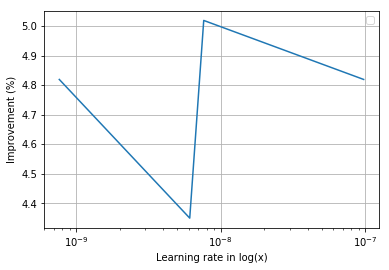
\includegraphics[width=.5\textwidth]{assets/appendix/plot_group25.png}
    \caption{Without batch normalization}
    \label{fig:ch_5_plot25}
\end{figure}
\begin{figure}[h]
    \centering
    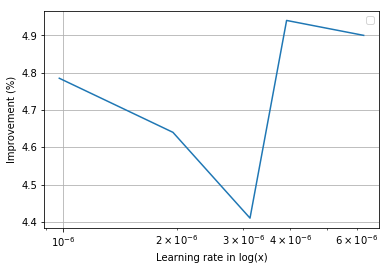
\includegraphics[width=.5\textwidth]{assets/appendix/plot_group21.png}
    \caption{With batch normalization}
    \label{fig:ch_5_plot21}
\end{figure}
\begin{figure}[h]
    \centering
    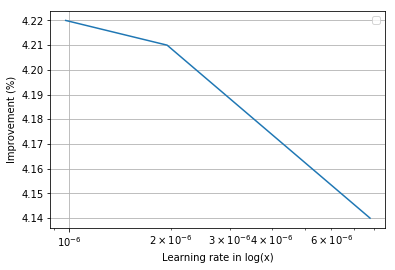
\includegraphics[width=.65\textwidth]{assets/appendix/plot_group23.png}
    \caption{Without batch normalization}
    \label{fig:ch_5_plot25}
\end{figure}
\begin{figure}[h]
    \centering
    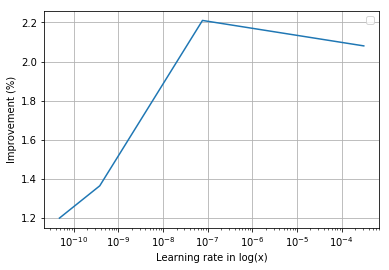
\includegraphics[width=.65\textwidth]{assets/appendix/plot_group1.png}
    \caption{Without batch normalization}
    \label{fig:ch_5_plot1}
\end{figure}
\begin{figure}[h]
    \centering
    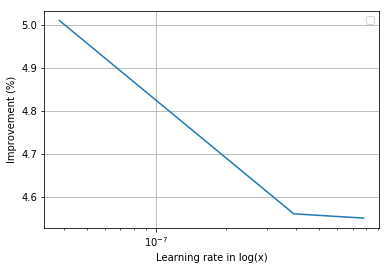
\includegraphics[width=.65\textwidth]{assets/appendix/plot_group5.png}
    \caption{Without batch normalization}
    \label{fig:ch_5_plot5}
\end{figure}

\chapter{Most significant variables according to feature selection}
The following tables list the variables that best correlate with labeled output and may therefore possess potentially good discrimination capabilities. They were determined using the various feature selection algorithms introduced in Section \ref{sec:ch-5-input-vars}.

\npdecimalsign{.}
\nprounddigits{2}

\LTXtable{\textwidth}{assets/appendix/anova}
\LTXtable{\textwidth}{assets/appendix/rfe}
\LTXtable{\textwidth}{assets/appendix/fi}
